\documentclass[12pt,a4paper]{article}

\usepackage[margin=1in]{geometry}
\usepackage{graphicx}
\usepackage{booktabs}
\usepackage{array}
\usepackage{amsmath}
\usepackage{xcolor}
\usepackage{listings}
\usepackage{tikz}
\usetikzlibrary{shapes.geometric, arrows.meta, positioning, calc}
\usepackage{fancyhdr}
\usepackage{setspace}
\usepackage[colorlinks=true,linkcolor=black,urlcolor=blue]{hyperref}

\setstretch{1.15}
\pagestyle{fancy}
\fancyhf{}
\lhead{Object Following Car}
\rhead{EEE Project Report}
\cfoot{\thepage}

% ---------- Code listing style ----------
\definecolor{cmt}{rgb}{0.0,0.5,0.0}
\definecolor{kw}{rgb}{0.0,0.0,0.7}
\lstdefinestyle{arduino}{
  language=C++,
  basicstyle=\ttfamily\footnotesize,
  keywordstyle=\color{kw}\bfseries,
  commentstyle=\color{cmt}\itshape,
  numbers=left,
  numberstyle=\tiny,
  numbersep=6pt,
  frame=single,
  breaklines=true,
  tabsize=2,
  showstringspaces=false
}
\lstset{style=arduino}

\begin{document}

% ================= TITLE PAGE =================
\begin{titlepage}
\centering
{\Large \textbf{[Sylhet International University]}}\\[0.3cm]
{\large Department of Computer Science and Engineering}\\[2cm]

{\Huge \textbf{Object Following Car}}\\[0.6cm]
{\large Using Arduino Uno, Ultrasonic Sensor and IR Sensors}\\[1.5cm]

{\large \textbf{Project Report}}\\[0.3cm]
{\large Course Code: [EEE 0714-211] \quad Course Title: [Electronic Devices and Circuits]}\\[1.8cm]

\textbf{\large Submitted By (Project Members)}\\[0.4cm]
\begin{tabular}{rl}
1. & Abir \\
2. & Arif \\
3. & Mamun \\
4. & Shanto \\
5. & Plaboni \\
6. & Nasifa \\
7. & Azhar \\
\end{tabular}\\[0.3cm]

\textbf{\large Submitted To}\\[0.3cm]
[Tasnim Rahman Zamee]\\
Designation\\
Department of Computer Science and Engineering\\[1.5cm]

Date of Submission: [03-11-2026]
\end{titlepage}

% ================= 1. INTRODUCTION =================
\section{Introduction}
Autonomous mobile robots are widely used in industry, logistics, surveillance, healthcare and domestic automation. A basic capability of such robots is to sense the environment and respond to it without human control. One of the simplest and most useful behaviours is \emph{object following}, where the robot keeps track of a target and moves with it.

This project implements an object following car using low-cost and easily available components. A microcontroller reads the distance to an object from an ultrasonic sensor and the presence of objects at the left and right sides from two IR sensors, and then drives four DC motors through a motor shield to move forward, turn left, turn right or stop.

\subsection{Objectives}
The main objectives of this project are:
\begin{itemize}
  \item To design and build a four-wheel robot car that can follow an object placed in front of it.
  \item To interface an ultrasonic sensor and IR sensors with an Arduino Uno.
  \item To control four DC motors using an L293D motor shield.
  \item To develop and test the control program in the Arduino IDE.
  \item To gain practical experience in sensors, embedded systems and robotics.
\end{itemize}

\subsection{Scope and Applications}
The same principle can be extended to shopping-cart robots, person-following luggage carriers, warehouse transport vehicles, line and obstacle based guided vehicles, and educational robotics platforms.

% ================= 2. COMPONENTS =================
\section{Components Used}
Table~\ref{tab:components} lists the hardware used in this project.

\begin{table}[h]
\centering
\caption{List of components}
\label{tab:components}
\begin{tabular}{@{}clc@{}}
\toprule
\textbf{S/N} & \textbf{Component} & \textbf{Quantity} \\
\midrule
1 & Arduino Uno R3 & 1 \\
2 & Servo Motor SG90 & 1 \\
3 & 4-Wheel Robot Chassis Kit (with 4 DC gear motors) & 1 \\
4 & L293D Motor Driver Shield & 1 \\
5 & HC-SR04 Ultrasonic Distance Sensor Module & 1 \\
6 & IR Sensor Module FC-51 & 2 \\
7 & 2-Chamber 18650 Battery Holder & 1 \\
8 & 18650 Li-ion Battery & 2 \\
9 & Jumper Cables & As required \\
10 & Switch, connecting wires and other accessories & As required \\
\bottomrule
\end{tabular}
\end{table}

\subsection{Arduino Uno R3}
The Arduino Uno R3 is based on the ATmega328P microcontroller. It has 14 digital input/output pins (6 of which provide PWM), 6 analog inputs, a 16~MHz crystal oscillator, USB connection and a power jack. It operates at 5~V logic level and acts as the brain of the car: it reads the sensors and decides the motor actions.

\subsection{L293D Motor Driver Shield}
The L293D shield stacks directly on the Arduino Uno and carries two L293D dual H-bridge drivers and a 74HC595 shift register. It can drive up to four DC motors with individual speed control (via PWM) and direction control, and up to two servo motors. The \texttt{AFMotor} library is used to control it. Because an Arduino pin cannot supply enough current for a motor, the shield acts as a power interface between the microcontroller and the motors.

\subsection{HC-SR04 Ultrasonic Sensor}
The HC-SR04 measures distance by emitting a 40~kHz ultrasonic burst and timing the echo that returns from an object. It operates at 5~V and has an effective range of about 2~cm to 400~cm. The distance is calculated as
\begin{equation}
d = \frac{v \times t}{2}
\end{equation}
where $v \approx 343$~m/s is the speed of sound in air at room temperature, $t$ is the echo time and the division by 2 accounts for the round trip of the sound wave. In this project the \texttt{NewPing} library is used with a maximum range of 200~cm.

\subsection{FC-51 IR Sensor Module}
The FC-51 consists of an infrared LED transmitter and a photodiode receiver with an LM393 comparator. When an object is within its detection range (about 2--30~cm, adjustable using the on-board potentiometer), IR light is reflected to the receiver and the digital output goes \textbf{LOW} (0). With no object, the output stays \textbf{HIGH} (1). Two such modules are used, one for the right side and one for the left side.

\subsection{Servo Motor SG90}
The SG90 is a small 9~g servo with about 180$^\circ$ rotation, operated from 4.8--6~V and controlled by a PWM signal. In this project it carries the ultrasonic sensor mounting position and is attached to pin~10; it is swept once at start-up as a self-test.

\subsection{4-Wheel Robot Chassis Kit}
The chassis kit provides the acrylic body, four wheels and four DC gear (TT) motors on which all other components are mounted.

\subsection{18650 Batteries and Holder}
Two 18650 Li-ion cells (3.7~V nominal each) in a 2-chamber holder are connected in series to give approximately 7.4~V, which powers the motor shield, motors and Arduino. The 18650 cells have a high energy density and can supply the current required by four motors.

% ================= 3. SYSTEM DESIGN =================
\section{System Design}

\subsection{Block Diagram}
Figure~\ref{fig:block} shows the block diagram of the system. The ultrasonic and IR sensors send data to the Arduino, which processes it and commands the motor driver shield to run the four DC motors.

\begin{figure}[h]
\centering
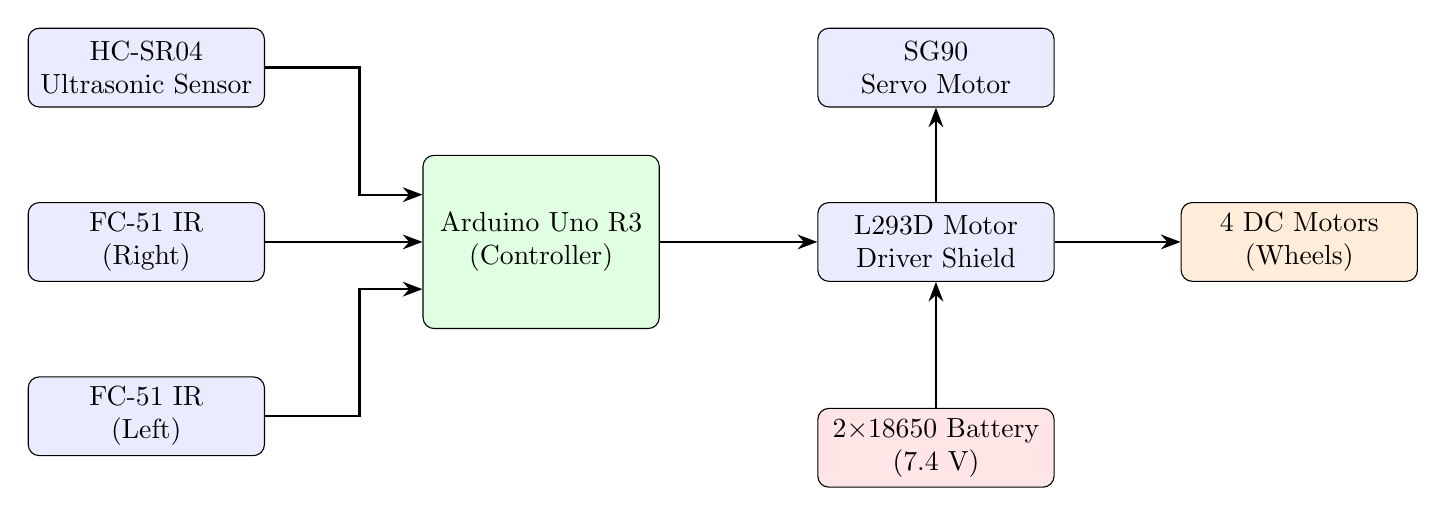
\begin{tikzpicture}[
  node distance=1.2cm and 1.6cm,
  box/.style={rectangle, draw, rounded corners, minimum width=3cm, minimum height=1cm, align=center, fill=blue!8},
  arr/.style={-{Stealth[length=2.5mm]}, thick}
]
\node[box] (us) {HC-SR04\\Ultrasonic Sensor};
\node[box, below=of us] (irr) {FC-51 IR\\(Right)};
\node[box, below=of irr] (irl) {FC-51 IR\\(Left)};
\node[box, right=2cm of irr, fill=green!12, minimum height=2.2cm] (ard) {Arduino Uno R3\\(Controller)};
\node[box, right=2cm of ard] (drv) {L293D Motor\\Driver Shield};
\node[box, right=1.6cm of drv, fill=orange!15] (mot) {4 DC Motors\\(Wheels)};
\node[box, above=of drv] (srv) {SG90\\Servo Motor};
\node[box, below=1.6cm of drv, fill=red!10] (bat) {2$\times$18650 Battery\\(7.4 V)};

\draw[arr] (us.east) -| ($(ard.west)+(-0.8,0.6)$) -- ($(ard.west)+(0,0.6)$);
\draw[arr] (irr.east) -- (ard.west);
\draw[arr] (irl.east) -| ($(ard.west)+(-0.8,-0.6)$) -- ($(ard.west)+(0,-0.6)$);
\draw[arr] (ard.east) -- (drv.west);
\draw[arr] (drv.east) -- (mot.west);
\draw[arr] (drv.north) -- (srv.south);
\draw[arr] (bat.north) -- (drv.south);
\end{tikzpicture}
\caption{Block diagram of the object following car}
\label{fig:block}
\end{figure}

\subsection{Pin Connections}
Table~\ref{tab:pins} summarizes the connections between the Arduino and the peripherals as defined in the program.

\begin{table}[h]
\centering
\caption{Pin connections}
\label{tab:pins}
\begin{tabular}{@{}lll@{}}
\toprule
\textbf{Device} & \textbf{Device Pin} & \textbf{Arduino Pin} \\
\midrule
HC-SR04 & Trigger & A1 \\
HC-SR04 & Echo & A0 \\
HC-SR04 & VCC / GND & 5V / GND \\
IR Sensor (Right) & OUT & A2 \\
IR Sensor (Left) & OUT & A3 \\
IR Sensors & VCC / GND & 5V / GND \\
Servo SG90 & Signal & D10 (Servo 1 header on shield) \\
DC Motor 1 & M1 terminal & Motor shield M1 \\
DC Motor 2 & M2 terminal & Motor shield M2 \\
DC Motor 3 & M3 terminal & Motor shield M3 \\
DC Motor 4 & M4 terminal & Motor shield M4 \\
Battery (7.4 V) & + / $-$ & Motor shield external power terminal \\
\bottomrule
\end{tabular}
\end{table}

\subsection{Working Principle}
The car continuously performs the following operations:
\begin{enumerate}
  \item The ultrasonic sensor measures the distance $d$ to the object in front of the car.
  \item The two IR sensors check whether an object is detected on the right or on the left.
  \item If $1 < d < 15$~cm, the object is directly in front and close, so all four motors rotate forward at speed 130 (out of 255) and the car follows the object.
  \item Otherwise, if only the left IR sensor sees an object (Right $=0$, Left $=1$ in the program's logic), the car performs a left turn for 150~ms by rotating the left-side motors forward and right-side motors backward as coded.
  \item Otherwise, if only the right IR sensor sees an object (Right $=1$, Left $=0$), the car performs a right turn for 150~ms.
  \item Otherwise, if $d > 15$~cm, the object is out of following range, so all motors are released and the car stops.
\end{enumerate}

\begin{table}[h]
\centering
\caption{Control logic of the car}
\label{tab:logic}
\begin{tabular}{@{}cccl@{}}
\toprule
\textbf{Distance (cm)} & \textbf{Right IR} & \textbf{Left IR} & \textbf{Action} \\
\midrule
$1 < d < 15$ & X & X & Move forward (speed 130) \\
Otherwise & 0 & 1 & Turn left (speed 150, 150 ms) \\
Otherwise & 1 & 0 & Turn right (speed 150, 150 ms) \\
$d > 15$ & other & other & Stop \\
\bottomrule
\end{tabular}
\end{table}

\subsection{Flowchart}
\begin{figure}[h]
\centering
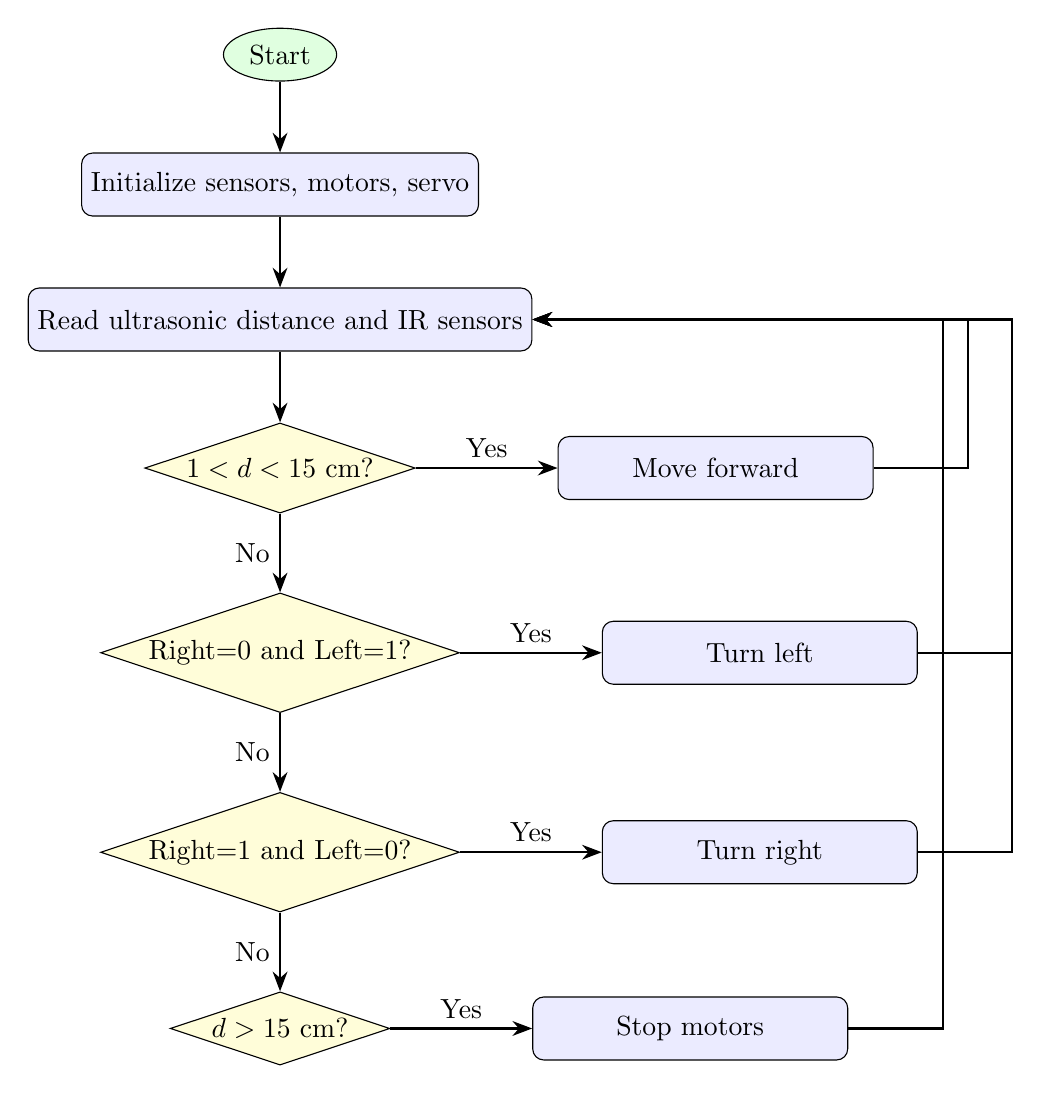
\begin{tikzpicture}[
  node distance=0.9cm,
  proc/.style={rectangle, draw, rounded corners, minimum width=4cm, minimum height=0.8cm, align=center, fill=blue!8},
  dec/.style={diamond, draw, aspect=3, align=center, fill=yellow!15, inner sep=1pt},
  term/.style={ellipse, draw, fill=green!12, align=center},
  arr/.style={-{Stealth[length=2.5mm]}, thick}
]
\node[term] (start) {Start};
\node[proc, below=of start] (init) {Initialize sensors, motors, servo};
\node[proc, below=of init] (read) {Read ultrasonic distance and IR sensors};
\node[dec, below=of read] (d1) {$1<d<15$ cm?};
\node[proc, right=1.8cm of d1] (fwd) {Move forward};
\node[dec, below=1cm of d1] (d2) {Right=0 and Left=1?};
\node[proc, right=1.8cm of d2] (left) {Turn left};
\node[dec, below=1cm of d2] (d3) {Right=1 and Left=0?};
\node[proc, right=1.8cm of d3] (right) {Turn right};
\node[dec, below=1cm of d3] (d4) {$d>15$ cm?};
\node[proc, right=1.8cm of d4] (stop) {Stop motors};

\draw[arr] (start) -- (init);
\draw[arr] (init) -- (read);
\draw[arr] (read) -- (d1);
\draw[arr] (d1) -- node[above]{Yes} (fwd);
\draw[arr] (d1) -- node[left]{No} (d2);
\draw[arr] (d2) -- node[above]{Yes} (left);
\draw[arr] (d2) -- node[left]{No} (d3);
\draw[arr] (d3) -- node[above]{Yes} (right);
\draw[arr] (d3) -- node[left]{No} (d4);
\draw[arr] (d4) -- node[above]{Yes} (stop);
\draw[arr] (fwd.east) -- ++(1.2,0) |- (read.east);
\draw[arr] (left.east) -- ++(1.2,0) |- (read.east);
\draw[arr] (right.east) -- ++(1.2,0) |- (read.east);
\draw[arr] (stop.east) -- ++(1.2,0) |- (read.east);
\end{tikzpicture}
\caption{Flowchart of the control program}
\label{fig:flow}
\end{figure}

% ================= 4. SOFTWARE =================
\section{Software Implementation}
The program is written in the Arduino IDE (C/C++). The following libraries are used:
\begin{itemize}
  \item \texttt{NewPing.h} -- reads the HC-SR04 sensor reliably and returns distance in cm.
  \item \texttt{Servo.h} -- generates the PWM signal for the SG90 servo.
  \item \texttt{AFMotor.h} -- controls the L293D motor shield (Adafruit Motor Shield library).
\end{itemize}

\subsection{Program Structure}
\begin{description}
  \item[Initialization] Pin definitions, sensor object (\texttt{sonar}), four motor objects (\texttt{Motor1}--\texttt{Motor4}) and the servo object are created. In \texttt{setup()}, serial communication is started at 9600~baud, the servo is attached to pin~10 and swept through $90^\circ \rightarrow 180^\circ \rightarrow 0^\circ \rightarrow 90^\circ$, and the IR pins are set as inputs.
  \item[Main loop] Every cycle waits 50~ms, reads the ultrasonic distance and both IR sensors, prints the values on the serial monitor for debugging, and then applies the decision logic described in Table~\ref{tab:logic}.
\end{description}

The complete source code is given in Appendix~A.

% ================= 5. CIRCUIT & ASSEMBLY =================
\section{Circuit Assembly}
\begin{enumerate}
  \item The four DC motors were fixed to the chassis and wheels were attached.
  \item The L293D motor shield was mounted on top of the Arduino Uno.
  \item Motors were connected to the shield terminals M1--M4.
  \item The HC-SR04 was fixed at the front of the car and connected to A0 (Echo) and A1 (Trigger).
  \item The two FC-51 IR sensors were placed at the front-right and front-left corners and connected to A2 and A3.
  \item The SG90 servo was connected to the servo header (pin 10).
  \item The two 18650 cells were placed in the holder (series, about 7.4~V) and connected to the shield's external power terminal through a switch.
\end{enumerate}

% ================= 6. RESULTS =================
\section{Results and Discussion}
The car was tested with a hand and a flat board as the target object.
\begin{itemize}
  \item When the object was placed between 1~cm and 15~cm in front, the car moved forward and followed it.
  \item When the object was moved away beyond 15~cm, the car stopped.
  \item When an object approached only one side, the corresponding IR sensor triggered and the car turned for a short time.
  \item Sensor readings were displayed on the serial monitor at 9600~baud, which helped in calibration.
\end{itemize}

\subsection{Observations and Limitations}
\begin{itemize}
  \item The FC-51 IR sensors are affected by strong sunlight and by the colour/reflectivity of the object, so indoor testing gives better results.
  \item The HC-SR04 has a narrow effective beam angle; soft or angled surfaces can give unreliable echoes.
  \item The following range is short (under 15~cm); increasing the distance threshold would allow a larger following distance.
  \item Battery voltage drop reduces motor speed over time.
  \item The servo is used only for a start-up sweep; it could be used to scan left and right with the ultrasonic sensor for better tracking.
\end{itemize}

% ================= 7. CONCLUSION =================
\section{Conclusion and Future Work}
An object following car was successfully designed and built using an Arduino Uno, an L293D motor shield, an HC-SR04 ultrasonic sensor and two FC-51 IR sensors. The robot detects an object ahead, follows it while it is within range, steers using side sensors and stops when the object leaves the range. The project provided hands-on experience in sensor interfacing, motor driving, embedded programming and system integration.

\textbf{Future improvements} include:
\begin{itemize}
  \item Using the servo to rotate the ultrasonic sensor for wider scanning.
  \item Adding a PID controller for smooth speed and distance control.
  \item Adding Bluetooth/Wi-Fi control and a mobile app.
  \item Using a camera with computer vision for person or colour tracking.
  \item Adding a battery level indicator and obstacle avoidance mode.
\end{itemize}

% ================= REFERENCES =================
\section*{References}
\addcontentsline{toc}{section}{References}
\begin{enumerate}
  \item Arduino, ``Arduino Uno Rev3 Documentation,'' \url{https://docs.arduino.cc}.
  \item Adafruit, ``Adafruit Motor Shield Library (AFMotor).''
  \item T. Eckel, ``NewPing Library for Arduino.''
  \item ``HC-SR04 Ultrasonic Sensor Datasheet.''
  \item Texas Instruments, ``L293D Quadruple Half-H Drivers Datasheet.''
  \item ``FC-51 Infrared Obstacle Avoidance Sensor Module Datasheet.''
\end{enumerate}

% ================= APPENDIX =================
\newpage
\appendix
\section{Complete Arduino Source Code}
\begin{lstlisting}
#include<NewPing.h>
#include<Servo.h>
#include<AFMotor.h>

#define RIGHT A2           // Right IR sensor
#define LEFT A3            // Left IR sensor
#define TRIGGER_PIN A1     // Ultrasonic trigger
#define ECHO_PIN A0        // Ultrasonic echo
#define MAX_DISTANCE 200   // Maximum ping distance

unsigned int distance = 0;
unsigned int Right_Value = 0;
unsigned int Left_Value = 0;

NewPing sonar(TRIGGER_PIN, ECHO_PIN, MAX_DISTANCE);

AF_DCMotor Motor1(1,MOTOR12_1KHZ);
AF_DCMotor Motor2(2,MOTOR12_1KHZ);
AF_DCMotor Motor3(3,MOTOR34_1KHZ);
AF_DCMotor Motor4(4,MOTOR34_1KHZ);

Servo myservo;
int pos=0;

void setup() {
  Serial.begin(9600);
  myservo.attach(10);

  for(pos = 90; pos <= 180; pos += 1){
    myservo.write(pos);
    delay(15);
  }
  for(pos = 180; pos >= 0; pos -= 1){
    myservo.write(pos);
    delay(15);
  }
  for(pos = 0; pos <= 90; pos += 1){
    myservo.write(pos);
    delay(15);
  }

  pinMode(RIGHT, INPUT);
  pinMode(LEFT, INPUT);
}

void loop() {
  delay(50);
  distance = sonar.ping_cm();
  Serial.print("distance");
  Serial.println(distance);

  Right_Value = digitalRead(RIGHT);
  Left_Value = digitalRead(LEFT);

  Serial.print("RIGHT");
  Serial.println(Right_Value);
  Serial.print("LEFT");
  Serial.println(Left_Value);

  if((distance > 1) && (distance < 15)){
    // Move Forward
    Motor1.setSpeed(130); Motor1.run(FORWARD);
    Motor2.setSpeed(130); Motor2.run(FORWARD);
    Motor3.setSpeed(130); Motor3.run(FORWARD);
    Motor4.setSpeed(130); Motor4.run(FORWARD);

  }else if((Right_Value==0) && (Left_Value==1)){
    // Turn Left
    Motor1.setSpeed(150); Motor1.run(FORWARD);
    Motor2.setSpeed(150); Motor2.run(FORWARD);
    Motor3.setSpeed(150); Motor3.run(BACKWARD);
    Motor4.setSpeed(150); Motor4.run(BACKWARD);
    delay(150);

  }else if((Right_Value==1) && (Left_Value==0)){
    // Turn Right
    Motor1.setSpeed(150); Motor1.run(BACKWARD);
    Motor2.setSpeed(150); Motor2.run(BACKWARD);
    Motor3.setSpeed(150); Motor3.run(FORWARD);
    Motor4.setSpeed(150); Motor4.run(FORWARD);
    delay(150);

  }else if(distance > 15){
    // Stop
    Motor1.setSpeed(0); Motor1.run(RELEASE);
    Motor2.setSpeed(0); Motor2.run(RELEASE);
    Motor3.setSpeed(0); Motor3.run(RELEASE);
    Motor4.setSpeed(0); Motor4.run(RELEASE);
  }
}
\end{lstlisting}

\end{document}
